%%% Local Variables: 
%%% mode: latex
%%% TeX-master: "../master.tex"
%%% LaTeX-command: "latex -shell-escape"
%%% End:

\chapter{Union-Find}
%%%%%%%%%%%%%%%%%%%%%%%%%%%%%%%%%%%%%%%%%%%%%%%%
\section{Dynamic Connectivity}
\subsection{Applications involve manipulating objects of all types}
\begin{itemize}
 \item Pixels in a digital photo
 \item Computers in a network
 \item Friends in a social network.
 \item Transistors in a computer chip
 \item Variable name in Fortran program
 \item Metallic sites in a composite system
\end{itemize}

\vspace{10 mm}

\textbf{Given a set of N objects}
\begin{description}
  \item[Union command:] connect two objects
  \item[Find/connected query:] is there a path connecting the two objects?
\end{description}

\begin{figure}[h]
   \centering
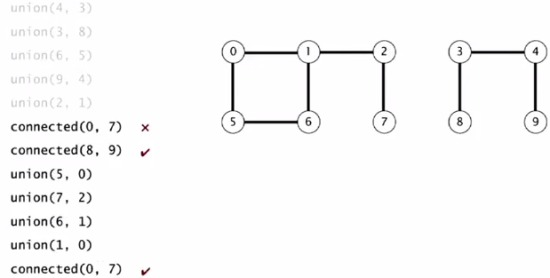
\includegraphics[scale=0.4]{tex_files/images/dynamicconnectivity.jpg}
\end{figure}



\vspace{10 mm}

\subsection{Implementing the operations}
\begin{description}
  \item[Find Query] Check if two objects are in the same component.
  \item[Union Command] Replace components containing two objects with their union.
\end{description}
For example if you have [0][1 4 5][2 3 6 7] where each [X...X] represents the connectec components if you use the operation \textbf{union(2,5)}
you will have [0][1 2 3 4 5 6 7]


\subsection{Union-find data type (API)}

\textbf{Goal} Design efficient data structure for union-find.
\begin{itemize}
\item Number of objects N can be huge.
\item Number of operations M can be huge.
\item Find queries and union commands may be intermixed.
\end{itemize}


\begin{table}[h]
\begin{center}
\begin{tabular}{cc}
\textbf{Public Class UF}        & \multicolumn{1}{l}{}                                          \\ \hline
UF(int N)                       & initialize union-find data structure with N objects(0 to N-1) \\ \hline
void union( int p, int q)       & add connection between p and q                                \\ \hline
boolean connected(int p, int q) & are p and q in the same component ?                           \\ \hline
int find(int p)                 & component identifier for p(0 to N-1)                          \\ \hline
int count()                     & number of components                                          \\ \hline
\end{tabular}
\end{center}
\end{table}

%%%%%%%%%%%%%%%%%%%%%%%%%%%%%%%%%%%%%%%%%%%%%%%%%%%%%%%%%%%%%%%%%%%%%%%%%%%%%%%%%%%%%%%%%%%%%%%%%%%%%%%%%%%%%%%%%%%%%%%%%%%%%%%%%%%%%%%%
\section{Quick Find}

\textbf{Data Structure}
\begin{itemize}
\item Integer array id[] of size N.
\item Interpretation: p and q are connected if they have the same id.
\end{itemize}
% \begin{minted}
% [
% frame=lines,
% framesep=2mm,
% baselinestretch=1.2,
% bgcolor=white,
% fontsize=\footnotesize,
% linenos
% ]
% {java}
% import numpy as np

% def incmatrix(genl1,genl2):
% m = len(genl1)
% n = len(genl2)
% M = None #to become the incidence matrix
% VT = np.zeros((n*m,1), int)  #dummy variable

% #compute the bitwise xor matrix
% M1 = bitxormatrix(genl1)
% M2 = np.triu(bitxormatrix(genl2),1) 

% for i in range(m-1):
% for j in range(i+1, m):
% [r,c] = np.where(M2 == M1[i,j])
% for k in range(len(r)):
% VT[(i)*n + r[k]] = 1;
% VT[(i)*n + c[k]] = 1;
% VT[(j)*n + r[k]] = 1;
% VT[(j)*n + c[k]] = 1;

% if M is None:
% M = np.copy(VT)
% else:
% M = np.concatenate((M, VT), 1)

% VT = np.zeros((n*m,1), int)

% return M
% \end{minted}

